% report template from https://www.overleaf.com/latex/templates/university-of-warwick-es327-cs351-report-template/nndyfbkvfvtm
% and inspied by Edmund Goodman

\documentclass[a4paper,fleqn,twoside,12pt]{report}

\usepackage[]{geometry}
\usepackage[latin1]{inputenc}
\usepackage[UKenglish]{babel}
\usepackage[UKenglish]{isodate}
\usepackage{amsmath}
\usepackage{amsfonts}
\usepackage{amssymb}
\usepackage{amsthm}
\usepackage{graphicx}
\usepackage{chngpage}
\usepackage{calc}
\PassOptionsToPackage{hyphens}{url}
\usepackage{hyperref}
\usepackage[nameinlink]{cleveref}
\usepackage{fancyhdr}
\usepackage{titletoc}
\usepackage[explicit]{titlesec}
\usepackage{natbib}
\usepackage[dvipsnames]{xcolor}
\usepackage[sc]{mathpazo}
\linespread{1.05}
\usepackage[T1]{fontenc}
\usepackage{minted}
\usepackage{graphicx}

%%%%%%%%%%%%%%%%%%%%

\hypersetup{
	colorlinks=true,
	linkcolor=black,
	urlcolor=black,
	citecolor=black
}

\setlength{\parindent}{0mm}
\setlength{\parskip}{\medskipamount}
\renewcommand\baselinestretch{1.2}

\cleanlookdateon

\makeatletter
\newcommand{\@assignment}[0]{Assignment}
\newcommand{\assignment}[1]{\renewcommand{\@assignment}{#1}}
\newcommand{\@supervisor}[0]{}
\newcommand{\supervisor}[1]{\renewcommand{\@supervisor}{#1}}
\newcommand{\@yearofstudy}[0]{}
\newcommand{\yearofstudy}[1]{\renewcommand{\@yearofstudy}{#1}}
\makeatletter

\author{Joel Coulon}
\title{Evaluating the Resiliency of Blink-Based DeepFake Detection Against\\Adversarial Noise}
\supervisor{Long Tran-Thanh}
\yearofstudy{3\textsuperscript{rd}}

%%%%%%%%%%%%%%%%%%%%

\pagestyle{plain}
\renewcommand{\headrulewidth}{0.0pt}

\makeatletter
\fancypagestyle{plain}{
	\fancyhf{}
	\fancyhead[LE]{\thepage}
	\fancyhead[RE]{\textit{\@author}}
	\fancyhead[RO]{\thepage}
	\fancyhead[LO]{\textit{\@title}}
}
\makeatother

%%%%%%%%%%%%%%%%%%%%

\begin{document}

\makeatletter
\newgeometry{margin=3cm}
\begin{titlepage}


    \textbf{\Huge \@title} \\[1.5cm]
    \Large \textbf{\@author} \\
    Department of Computer Science \\
    University of Warwick \\

    Supervised by \@supervisor \\
    Year of Study: \@yearofstudy \\

    \vfill

    \begin{adjustwidth}{-\oddsidemargin-1in}{-\rightmargin}
        \centering
        
\includegraphics[width=\paperwidth]{line.png}
    \end{adjustwidth}

    \vspace*{-2cm}

\end{titlepage}
\restoregeometry
\makeatother


\pagestyle{plain}

\pagenumbering{gobble}
\begin{abstract}
    Your abstract goes here. This should be about 2-3 paragraphs summarising the motivation for your project and the main outcomes (software, results, etc.) of your project. 
\end{abstract}

\renewcommand{\abstractname}{Acknowledgements}
\begin{abstract}
Hi Mum! {\tiny are you proud of me now?}
\end{abstract}

\pagenumbering{roman}
\tableofcontents
\listoffigures
\addcontentsline{toc}{chapter}{List of Figures}
\listoftables
\addcontentsline{toc}{chapter}{List of Tables}
\listoflistings
\addcontentsline{toc}{chapter}{List of Listings}
\newpage

\pagenumbering{arabic}
\chapter{Introduction}
\label{ch:introduction}

% \begin{itemize}
%     \item Introduction to deepfakes and a brief history
%     \item Mention things like initially coined on reddit, and their rise to popularity
%     \item can be used for a variety of illegal activities, misinformation, etc
%     \item adversarial noise
%     \item deepfake detection via CNNs 
%     \item the aim of the project
%     \begin{itemize}
%         \item the title but looong
%     \end{itemize}
%     \item objectives
%     \begin{itemize}
%         \item First objectives
%         \begin{enumerate}
%             \item Identify a methodology for detecting DeepFakes
%             \item Identify how to implement such a methodology
%             \item Implement such a methodology
%             \item Evaluate the feasibility of the produced method through standardised benchmarks
%         \end{enumerate}
%         \item{Optional (Extensions)}
%         Should all the essential objectives be completed the following could be implemented given sufficient time:
%         \begin{enumerate}
%             \item Enhance the chosen methodology through speed improvements, accuracy, etc.
%             \item Test the benefit of any potential improvement using standardised benchmarks
%         \end{enumerate}
%         \item New Objectives
%         \begin{enumerate}
%             \item Implement eye landmark detection
%             \item Calculate ear over time
%             \item analysis of ear graph to determine real or fake
%             \item implement a control set of models (state-of-the-art)
%             \item investigate and implement methods of adding adversarial noise
%             \item compare and benchmark over dataset(s)
%         \end{enumerate}
%         \item New Objectives (further)
%         \begin{enumerate}
%             \item Evaluate transferability of blink-detection across different datasets
%         \end{enumerate}
%     \end{itemize}\
%     \item Unique contributions
%     \begin{itemize}
%         \item First use of time series analysis on EAR graph
%         \item Evaluation of blink detection on standard datasets
%     \end{itemize}
% \end{itemize}

\section{Project Overview}
\label{sec:project-review}

DeepFakes are defined as ``manipulated or synthetic media whose realness is not easily recognisable by the human eye"\cite{altuncu2024deepfake}. In simpler terms, a DeepFake is a video, image, or audio clip that has been digitally altered or created, often using Artificial Intelligence (AI). Concerningly, it is extremely difficult for humans to determine whether or not a particular video has been DeepFaked. In a 2024 study, 86,155 volunteers attempted to detect DeepFakes, the final accuracy for all DeepFake types was 55.54\%\cite{diel2024human}, showing humans are only slightly better than guessing. Furthermore, a Europol report revealed that 72\% of the UK population were unaware of DeepFakes and their potential impact\cite{europol2022facing}.

\begin{figure}[h]
    \centering
    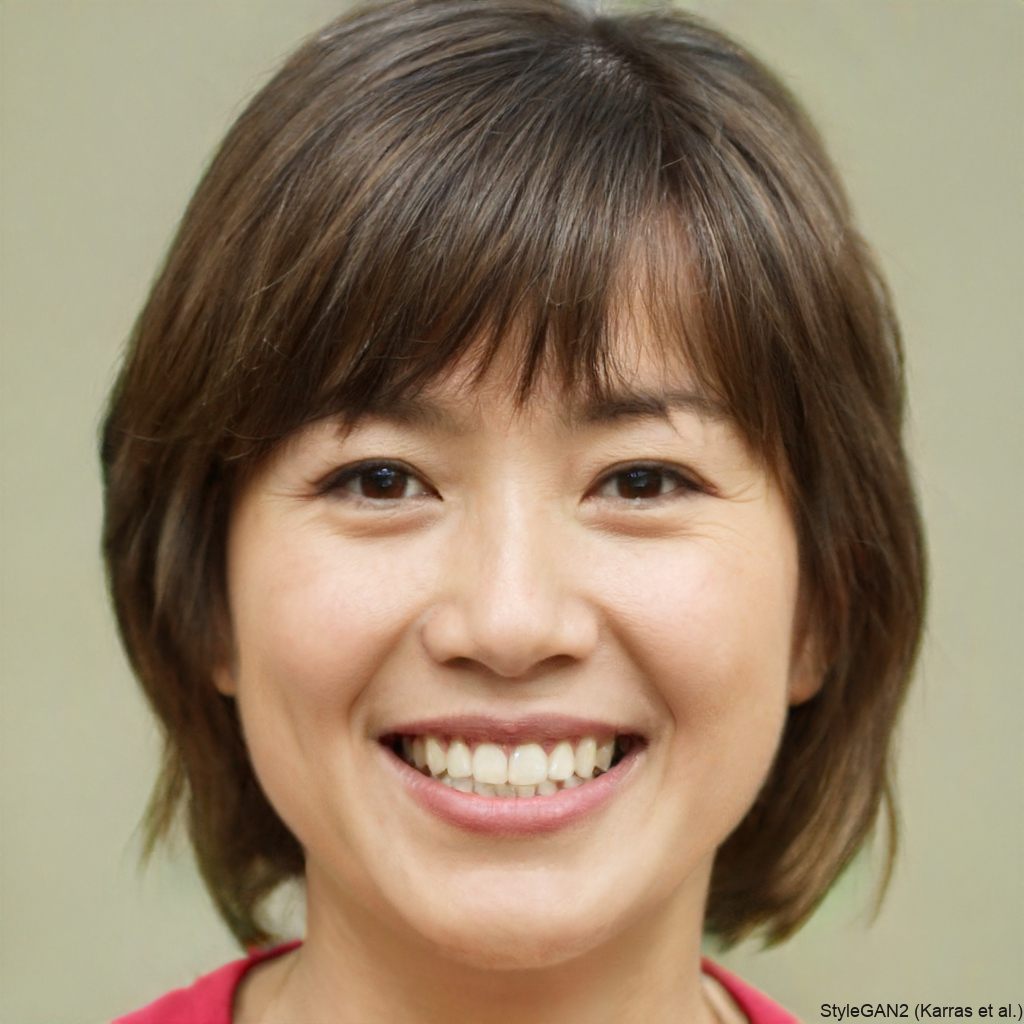
\includegraphics[width=0.5\linewidth]{dissertation//figures/thispersondoesnotexist.jpg}
    \caption{A DeepFake generated with \url{https://thispersondoesnotexist.com}}
    \label{fig:thispersondoesnotexist}
\end{figure}

Because they are so realistic, DeepFakes have garnered wide usage for various nefarious activities. Scams, misinformation, and fraud are all possible illegal uses of DeepFakes and all pose a real threat to society\cite{sensity2024state}. Deloitte estimates that in 2027, DeepFakes will enable more \$40 billion of fraud in the United States\cite{lalchand2024generative}.

It is therefore obvious that a mechanism to reliably detect DeepFakes would be incredibly useful.

Convolutional Neural Networks (CNNs) are powerful neural network models that learn kernels (sometimes also called filters) in a feed-forward manner\cite{lecun2015deep}. They consist of sequences of layers that gradually take a more and more general view of an input to produce the final classification. They have a wide variety of applications in various fields of deep learning, such as computer vision and recommendation algorithms. Crucially, they can also be used to create accurate DeepFake detectors. When trained on a specific dataset, they can become extremely accurate, achieving consistent accuracies of over 90\% when trained correctly\cite{papersiwthcodedeepfakedetection}.

However, recent studies have shown that CNNs are vulnerable to adversarial noise attacks. Noise, imperceptible to humans, is added to images which can cause a misclassification\cite{gandhi2020adversarial}. This becomes dangerous when noise is added to fake images, causing them to be classified as real. A 90\% accurate classifier is going to be implicitly trusted to be correct and a simple and invisible method to fool classifiers is worrying.

A promising new method of DeepFake detection focuses on blinking. DeepFakes and other AI-generated content suffer from various temporal inconsistencies. Videos are a sequence of images that move through time. When this video is real, certain aspects can be predicted between frames, however, AI struggles to replicate these aspects. Blink-based DeepFake detection exploits blinking inconsistencies. Human blinking is a subconscious action and hence periodic: the average period between blinks is 2.8 seconds and a blink takes around 0.1-0.4 seconds\cite{schiffman1990sensation}. Other eye-based temporal inconsistencies exist, such as the shape of an eye and how far open the eye can be. It is possible to leverage this for DeepFake detection, by analysing how far open the eye is over time.

This project aims to determine whether blink-based DeepFake detection is resistant to adversarial noise. It is believed to be resilient as blink-based detection classifies a video over time. Current methods of adversarial noise can only perturb a single frame at once and so, in theory, would not be able to coordinate to cause a misclassification overtime. However, adversarial attacks may cause landmarks to be mislocated. This may cause indirect misclassifications. 

This project also aims to evaluate whether blink-based detection can be used as a general DeepFake classifier or not. The majority of CNN-based detectors attain high accuracies by focussing on model-specific artifacts (Figure \ref{fig:fakeretouch}). On the other hand, the majority of DeepFakes will miss common factors in blinking such as frequency and period, and these patterns should be consistent across DeepFakes methodologies as similar kinds of mistakes will be made. Hence, it is believed that blink-based DeeepFake detectors will be generalised.

\section{Aim}
\label{sec:aim}

This paper aims to implement blink-based DeepFake detection and show that such a method is competitively resistant to adversarial noise attacks.

\section{Objectives}
\label{sec:objectives}

To achieve the aim, as laid out in Section \ref{sec:aim}, the project can be decomposed into the following objectives:

\begin{enumerate}
    \item Produce a method to reliably track how ``open" an eye is over time
    \item Analyse the resulting data to determine whether a video is fake or not, accurately
    \item Evaluate the performance of the model on standardised benchmarks
    \item Implement state-of-the-art traditional models
    \item Implement a variety of methods of adversarial noise to target those models
    \item Evaluate how responsive blink-based detection is to adversarial noise
\end{enumerate}

The above objectives must be completed for the project to be deemed a success. If they have all been successfully achieved, then the following objectives could be implemented given sufficient time:

\begin{enumerate}
    \item Evaluate the transferability of blink-based detection to datasets it has not been trained on
    \item Review possible noise reduction methods for DeepFake detection
\end{enumerate}

\section{Novel Contributions}
\label{sec:novel}

The project has the following novel contributions to the field of DeepFakes:

\begin{enumerate}
    \item First use of complex time series analysis for blink-based DeepFake detection
    \item First evaluation of blink-based DeepFake detection on common datasets
    \item First evaluation of transferability of blink-based DeepFake detection
\end{enumerate}
\chapter{Background}
\label{ch:background}

\section{Introduction to DeepFakes}

Hi DeepFakes, exist.

\section{DeepFake Detection}

You can detect them

\section{Adversarial Noise}

You can (successfully) fool them
\chapter{Design \& Implementation}
\label{ch:design-implementation}

\section{Language \& Libraries}

% \begin{itemize}
%     \item Python as pre-existing machine learning frameworks
%     \item Tensorflow vs PyTorch (Tensorflow seemed nicer and more base code, first code seen for proof of concept was in tensorflow)
%     \item mutually exclusive due to CUDA implementations
% \end{itemize}

\subsection{Python}

When choosing a language to code this project in Python\footnote{\url{https://www.python.org}} was a clear choice. Whilst other languages offer better speed (C++\footnote{\url{https://cplusplus.com/}}, Rust\footnote{\url{https://www.rust-lang.org/}}), Python's advantage comes from its libraries.

Libraries are modular pieces of code written by other developers that can be integrated into a new software to make common tasks easier. In Python this is accomplished using the \verb|import| and \verb|from| syntax. Libraries vastly simplify coding as they can vastly reduce complex problems to simple functions. This is especially useful when dealing with complex machine learning functions, advanced mathematical algorithms such as Adam can be reduced to an import. Many Python libraries are written in lower-level languages like C or C++, allowing Python code to benefit from high performance while maintaining ease of use.

The vast majority of popular packages have a Python implementation that can be easily installed by the Python Package Index\footnote{\url{https://pypi.org/}}. Especially for machine learning, Python has some of the largest collection of relevant libraries of any language and is therefore the language of choice for this project.

\subsection{PyTorch versus TensorFlow}

There are many machine learning frameworks in Python, however the primary two are PyTorch\cite{paszke2019pytorch} and TensorFlow\cite{abadi2016tensorflow}. They both offer near identical feature sets and performance so choosing between them is not a simple matter.

PyTorch was created by Meta in 2019. It is a lot newer and viewed as a more ``pythonic" framework\cite{chirodea2021comparison}. To be more ``pythonic" is to be more developer-friendlier by providing a simple interface to the library that developers already familiar with Python should easily pick up on. PyTorch supports a dynamic computation graph which enables for dynamic changes of model architectures.

TensorFlow is a much more mature framework by Google releasing in 2015. It offers similar abstractions as PyTorch but is widely viewed to be slightly harder to develop in\cite{chirodea2021comparison}. TensorFlow uses an eager computation graph meaning no changes to model architectures can be made once a model is defined. Whilst this reduces flexibility during runtime, it allows for more optimisations to be made to the model architecture meaning greater accuracy, smaller model architectures, and sometimes quicker computations. TensorFlow also scales effectively running as efficiently as possible on desktop computers to large GPU clusters.

Unfortunately, TensorFlow and PyTorch are mutually exclusive. Both rely on separate versions of the CUDA backend to allow for GPU acceleration on NVIDIA architectures. Whilst this can be accomplished using virtually environments and other work arounds it is generally recommended to use one or the other.

Due to their similarities, there is no clear choice between PyTorch and TensorFlow. Some trends have emerged, however, with PyTorch being used for research and development work where iterative improvements are desired whereas as TensorFlow is employed for production environments. 

TensorFlow was chosen for this project for a number of reasons. Firstly, the flexibility that PyTorch offers is less important to this project as all models being used have had their architectures pre-defined. On the other hand, TensorFlow's ability to scale and optimise for the compute resources will be valuable for this project as it will be developed on smaller desktops but the final evaluation loops will be run on large GPU clusters. Furthermore, after trying out both TensorFlow and PyTorch, the author preferred the overall syntax of TensorFlow.

\section{Proof of Concept}
\label{sec:concept-design}

% \begin{itemize}
%     \item Re-use oriented design
%     \item Quick and dirty
%     \item test my theory
%     \item explain methodologies
% \end{itemize}

To validate whether or not blink-based DeepFake detection is resistant to adversarial noise, it was decided to construct a proof of concept during the Christmas holiday. As it is intended to be a small test-bed, small flaws in the design are acceptable. Therefore, it makes sense to use pre-existing models, solutions, and implementations where possible in order to speed up development.

\subsection{Architecture}

The overall architecture of blink based DeepFake detection is relatively simple. First, the landmarks around the face are computed to determine for every frame to generated an EAR-time graph. The graph can then be analysed to determine whether the video is real or not.

It was decided to use an EAR-based approach over a custom blink model, because it allows for complex analysis. EAR data is more precise than the binary open/close of a custom model, allowing for analysis of not just frequency of blinks but more subtle details like how the blink starts and ends, the velocity of the eye, and whether the eye consistently returns to the same position when open. The flaws in EAR noted by Ictu Oculi\cite{li2018ictu} are valid but they rely on the eye landmarks being unreliably marked, with sufficiently advanced models trained with occlusions this can be overcome. 

To calculate the EAR, the six landmarks around the eye need to be located. Google's MediaPipe\cite{lugaresi2019mediapipe} was used for this purpose. It is designed to run in real-time on mobile devices and other edge compute resources and hence is very light weight and fast. MediaPipe produces 478 landmarks in three dimensions that cover the entire face, a subset of twelve (six landmarks per eye) is then used to be the six landmarks for EAR. From the six landmarks, the EAR can be calculated using Equation \ref{eq:ear} and the average taken for the final EAR-time graph. 

EAR analysis is done via hybrid of DeepVision\cite{jung2020deepvision} and Ictu Oculi\cite{li2018ictu} by counting the number of blinks in the EAR graph and comparing that to the human average. DeepVision's database was viewed as too time-consuming to produce and the simplicity of Ictu Oculi's approach was appealing for its speed advantage. In experiments, DeepVision's threshold of two standard deviations below the mean proved to be to inconsistent so a revised threshold of half a standard deviation above the minimum EAR value was chosen. The average human blinks 14 times per minute\cite{schiffman1990sensation}, DeepFakes will blink less than this and so if the subject of the video blinks less than 14 times a minute, the video is deemed as a fake.

For traditional detectors, both ResNet and VGG architectures have been proven vulnerable to adversarial noise\cite{gandhi2020adversarial}. A ResNet-based DeepFake detector was implemented using an implementation from Tiwari\cite{tiwari2024deepfake}, a VGG-detector was implemented using a header from Krishna et al\cite{krishna2022deepfake} but the backbone was upgraded to VGG19 following research from Yadav et al\cite{yadav2024deepfake}. To extend frame-by-frame detection to entire videos, each frame in a video is analysed individually. If the frame is classified as fake then a counter is incremented by one. If the counter exceeds a given threshold (set as one hundred frames), the video is classed as fake. 

Adversarial noise was added to images using the Foolbox library\cite{rauber2017foolbox}\cite{rauber2017foolboxnative}. FGSM was used as the method for noise due to its known effectiveness and speed\cite{gandhi2020adversarial}. $\epsilon$ was set to 0.1. To replicate real life scenarios, noise was only added to faked videos and all models were solely trained on original videos, not noisy ones.

Models were trained on a subset of fifty real and fifty fake videos from the FaceForensics++ dataset. Testing was run over a further fifty real and fifty fake videos. The results of the tests can be found in Section \ref{sec:concept-results}.

{\huge need to add datasets to lit review}

\section{Main Algorithm}

\begin{itemize}
    \item pseudocode of main algorithm
    \item if at any point something fails, mark as fake (ensures resiliency)
    \item emphasise each part is interchangeable
\end{itemize}

\subsection{Eye Landmark Detection}

\begin{itemize}
    \item EAR needs 6 points per eye so lets get them
    \item Facial landmarking is a common superset problem
    \item Introduce 68 landmarks and datasets
    \item Most popular ones aren't viable as built to be small to fit in a package (dlib, opencv...) or to run on a phone (mediapipe)
\end{itemize}

\subsubsection{Face cropping}

YuNet for first pass, MTCNN if yunet fails

\subsubsection{Weakly Supervised Eye Landmarks Detection (WSELD)}

\begin{itemize}
    \item Looked promising
    \item Most accurate according to landmarks in paper \& only model focussing specifically on eye landmarking
    \item Has a ``good enough" implementation details
    \item Had issues
    \begin{itemize}
        \item Landmarks from regions (mention other paper that managed it
        \item difficulty implementing in tensorflow
        \item after a month scrapped development
    \end{itemize}
\end{itemize}

\subsubsection{Pre-implemented Models}

\begin{itemize}
    \item Re-use oriented design
    \item papers with code
    \item Used best models which had pre-existing implementations (one for fast, one more accurate)
    \item couldve optimised for 6 landmarks but didnt want to mess with model architectures that were known working (batch size probably meant nothing would change anyway)
\end{itemize}

\subsubsection{HRNet}

\begin{itemize}
    \item modular sequences
    \item keeps high resolution layers in context at all times
    \item generic network but with a specific implementation for eye landmarking
    \item Heatmap per landmark
\end{itemize}

\subsubsection{PFLD}

\begin{itemize}
    \item speedy boi
    \item uses mobilenet-techniques to reduce the size and increase the speed
    \item still accurate tho
    \item secret sauce is custom loss function
\end{itemize}

\subsubsection{Facial Landmark Datasets}

\begin{itemize}
    \item 68 landmarks (upsampling and downsampling where necessary)
    \item list all of them and give brief overview
    \item didnt use aflw due to inaccurate landmarks or not enough landmarks
    \item reflected to double size
\end{itemize}

\subsubsection{Final model choice}

Yunet + PFLD, then MTCNN and HRNET as backup (hope ear analysis can filter out idiosyncrasies of the model as will be consistent across real and fake)

\subsection{EAR Analysis}

\begin{itemize}
    \item Can be abstracted to a univariate time series
    \item Well researched
    \item Classical methods exists (pyts library)
    \item explain each one and give simple summary (1 paragraph)
    \item As do deep learning frameworks (the other papers)
    \item model diagrams for each one (maybe give a rough explenation as to the aims each one is doing?)
\end{itemize}

\section{Adversarial Noise}

\begin{itemize}
    \item foolbox library (Targeted FGSM using the other thing)
    \item chosen over cleverhans as cleverhans had meh documentation
    \item cw-l2 attack too slow (3hrs per video)
    \item fakeretouch has no open-source implementation, timings were too slow, estimated would also take a while
\end{itemize}

\section{DeepFake Datasets}
\label{sec:datasets}

\section{Final Code}

\begin{itemize}
    \item One codebase to do full training, splitting and evaluation
    \item just give overall flow diagram?
    \item {\huge models only trained on non-noisy images}
    \item checkpointing where possible
    \item run on either dcs compute clusters or avon
    \item final speeds + hardware
\end{itemize}
\chapter{Results and Evaluation}
\label{ch:evaluation}

\section{Proof of Concept}
\label{sec:concept-results}

\begin{itemize}
    \item initial results good
    \item VGG19 was targeted and had was reduced to 0\% accuracy
    \item ResNet however was not impacted
    \item therefore noise is effective for the model it attacks
    \item however other models not affected, need to test further
    \item \url{https://github.com/Mole1424/3rd-year-project/tree/main/proof-of-concept}
\end{itemize}

\section{Main Code Results}

\begin{itemize}
    \item Initial results VERY promising
    \item custom model is consistently 56\% accurate
    \begin{itemize}
        \item less accurate than expected
        \item consistently accurate tho so shows that the method is viable
        \item for some reason every model chose learning shapelets as the best one
    \end{itemize}
    \item other models are very accurate (80-90\%)
    \item however get massively degraded when noise is added
    \item noise is transferable and so other models will be downgraded though not to the same extent
    \item custom model was never affected, in fact sometimes improved
    \item compare hrnet to pfld, hrnet is more accurate and so had better results
    \item very little change with $\epsilon$ for advarserial noise
    \item spam graphs, main results in table
    \item ``The presentation of the results needed to be more rigourous, e.g., considering other methods without blink detection and other data sets (e.g., not simply that adding noise increased accuracy for the blink method). Also needed clearer definition of acuracy, so you can be sure that your system is not just detecting noise - what are the results for real video as well as fake?"
\end{itemize}

Transferability results soonTM

\section{Main Code Evaluation}

\begin{itemize}
    \item mention potential downsides of blink based
    \begin{itemize}
        \item required eyes to be constantly visible for reliable detection
        \item requires eyes to be faked
    \end{itemize}
    \item obviously other adversarial noise methods need to be evaluated but ran out of time :(
\end{itemize}
\chapter{Conclusions}
\label{ch:conclusions}

Wrap this damn thing up

\section{Future work}



\bibliographystyle{ieeetran}
\bibliography{bibliography.bib}

\appendix
\chapter{Sample appendix}
An appendix is an organ on the human body

\end{document}